%\begin{figure*}[t]
%	
\includegraphics[width=\textwidth]{images/dog.jpg}
%	\caption{Woo such a cute dog.}
%	\label{figure:dog}
%	\centering
%\end{figure*}

%We can see a very cute dog in \autoref{figure:dog}. 
%Such a good boy!
%Here is a reference~\cite{jia2023kernel}.

\lstset{
    language=C
}

\begin{quote}
"Simplicity is prerequisite for reliability." \\
\hspace*{\fill} — Edsger W. Dijkstra
\end{quote}

The task for Milestone 1 was to implement the infrastructure for managing physical memory using Barrelfish's capability system. This entailed coming up with our own representation of physical memory and defining all memory operations in terms of this representation. This section explains the design of our representation.

\subsection*{A Model of Physical Memory}
In class, we discussed several approaches to modeling physical memory, including bitmaps, red-black and AVL trees, and a linked list. We decided to use a (singly) linked list representation for one reason and one reason only: simplicity. Given that this was the first milestone, each one of us was relatively unfamiliar with the codebase, thus we wanted to focus on a \textit{correct} solution rather than an \textit{optimal} one. We discuss improvements on our design in a later \autoref{Improvements}.

Each node in the linked list is tied to a single "free" RAM capability (these are passed on to the `init` dispatcher from the CPU Driver). A node can be in one of two states: \textit{free} or \textit{allocated} and stores the size of the free/allocated block. Note that while we do enforce that every node holds unique capability references and that these capabilities point to disjoint address ranges, we do not maintain any particular ordering of the nodes. 


% During the initialization of the memory manager, it is given "free" RAM capabilities. When memory is allocated, these capabilities are retyped into another type, but regardless of type, these new capabilities are "descendants" of the original RAM capabilities. Thus, we capture this parent-child relationship in our mm\_node representations. We have two level of capabilities in each mm\_node. If the node represents a free piece of RAM, the ref will point to the RAM it represents and the parent is set NULL because the ref is already pointing to the "parent" RAMs. If the node represents an allocated RAM/Frame, the ref points to the allocated cap. Now there is a parent RAM, which is the large block of RAM we are allocating from. The offset is based from the "parent" RAM.

\subsection*{Allocating Memory}
To allocate memory, we traverse our linked list to find a memory region that satisfies the allocation requirements, and retype the free RAM capability into another capability of the type specified during the memory manager initialization. Notice that capabilities for allocated memory regions are descendants of the free RAM capabilities. We capture this parent-child relationship in each node by storing a parent capability reference. This reference is set to \verb|NULL_CAP| if the node is free (i.e just points to the free RAM).

Allocation requests may have specific alignment requirements and varying sizes which often result in situations where the allocation starts at an offset from beginning of the free region. Moreover, allocation requests will likely be smaller than the size of the free region. To ensure we don't leak memory, we insert padding nodes to keep track of these fragments. \autoref{figure:mm} illustrates this process.

As to our allocation strategy, we employ the \textit{first-fit} policy. Again, we made this choice since it was simple and the resulting fragmentation isn't too bad for our purposes. We briefly explored a the more efficient \textit{buddy} allocation strategy but we postponed its implementation due to time constraints.

We would also like to point out a subtle bug that we faced when setting up memory allocation. Initially, upon an allocation, we used the same \verb|capref| in our node for that allocation as the one we returned to the calling process. This caused weird errors where our memory manager lost track of large chunks of memory for no apparent reason. The fix was to insert a call to \verb|cap_copy| to ensure the capabilities used internally in our list are not affected by the capability operations performed by the \verb|init| process.

\begin{figure}[h]
	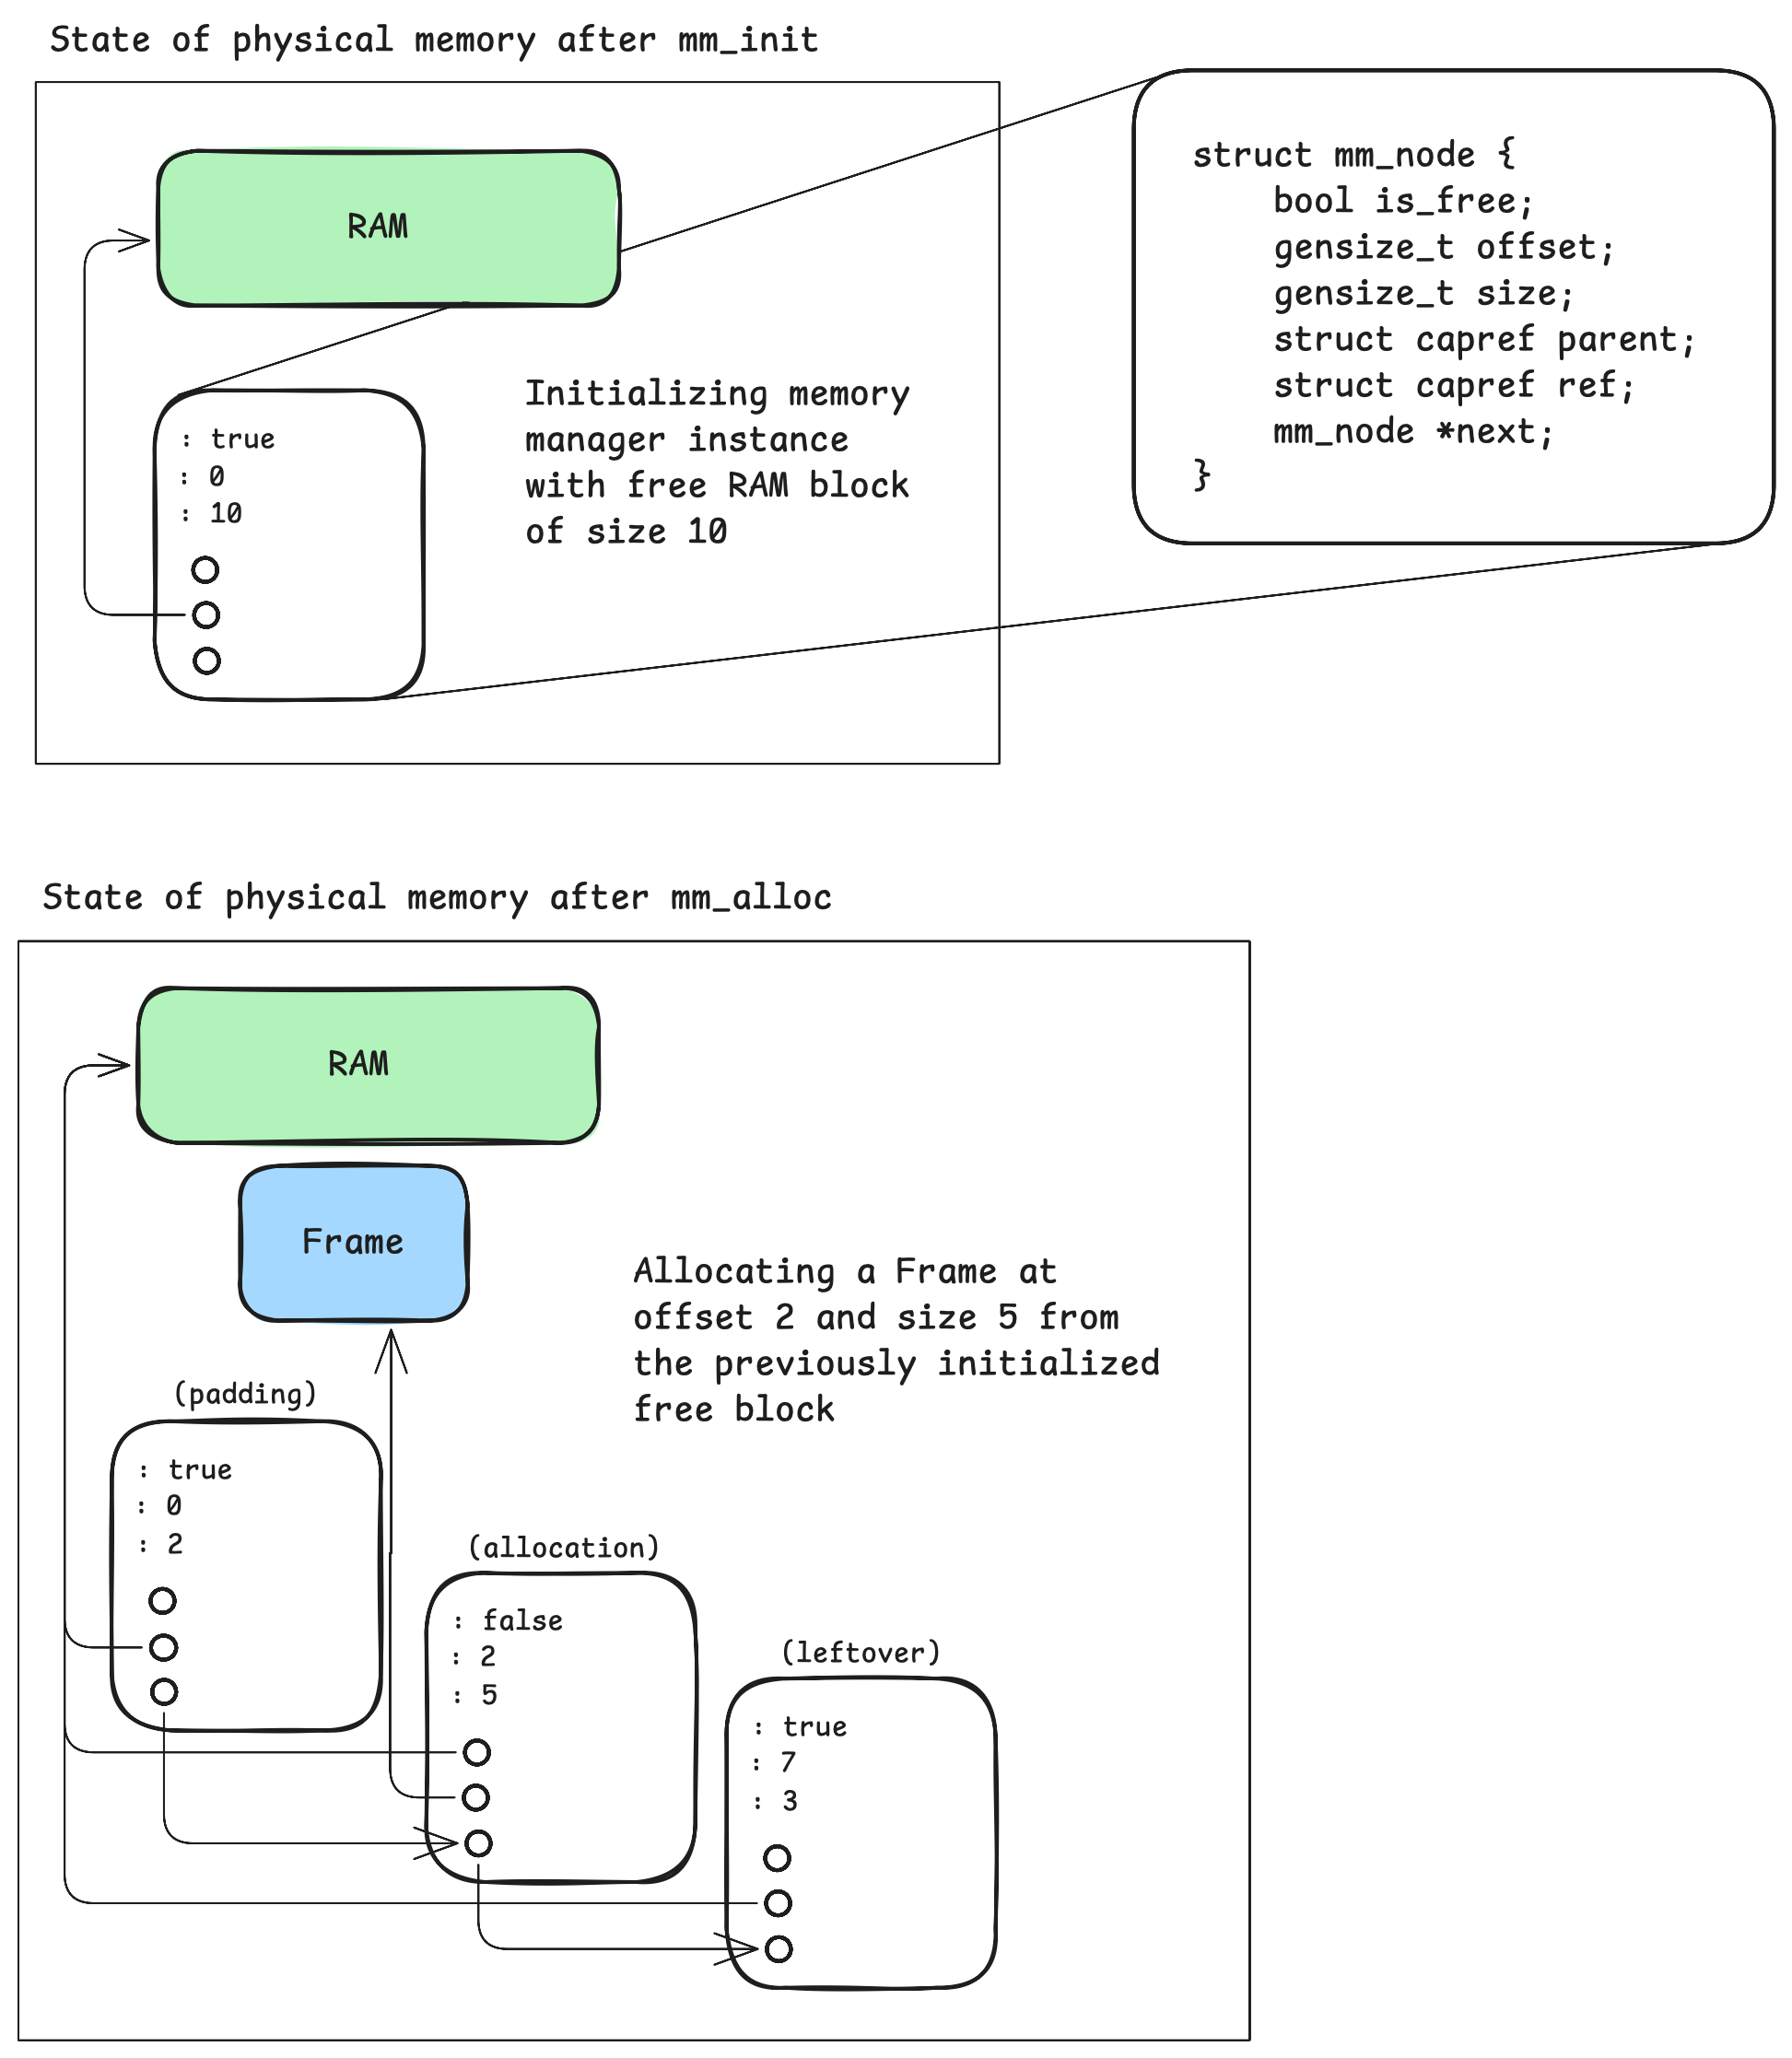
\includegraphics[width=\columnwidth]{report/images/mm-2.png}
	\caption{Keeping track of virtual memory regions}
	\label{figure:mm}
	\centering
\end{figure}

\subsection*{Freeing Memory}
Freeing previously allocated blocks of memory as a whole is essentially the inverse of allocating them and entails coalescing the padding/leftover nodes into a single node. Again, since we do not maintain any particular ordering of the nodes in our list, we are careful to not coalesce discontinuous memory regions.

Our implementation supports partial freeing of previously allocated blocks. To do so, we broke it down to following cases:
\begin{enumerate}
    \item The partially freed address range \textit{has the same start address} as its containing allocated range. In this case, we adjust the offset on the allocated node to align with the end address of the partially freed region. Note that we also call a retype on the allocated nodes's \verb|ref| capability to make sure it is updated to to refer to this new, smaller region of memory. We then create a new capability for the free region and call \verb|mm_add| to keep track of it.
    \item The partially freed address range \textit{has the same end address} as its containing allocated range. This case is identical to the previous one and is handled similarly -- the only difference here is that the "second half" is freed. This is taken into account when retyping capabilities and updating the pointers.
    \item The partially freed address range \textit{does not have the same start or end address} as its containing allocated range. In this case, the allocated region is split into three. The first and third regions are free and are added back into the memory manager by calls to \verb|mm_add| and the second region now refers to the smaller allocated region.
\end{enumerate}

Notice that since we make calls to \verb|mm_add| to keep track of the partially freed regions, once all sub-regions of an allocation are freed, we are unable to coalesce them. This is not ideal - we are essentially introducing "artificial" fragmentation. This may lead to a case where we are unable to satisfy an allocation request despite having enough memory since the representation of a free region is broken up into smaller pieces in our list.


% For the full deallocation, we simply find the node in the linked list and call cap\_destroy to the "ref" in the mm\_node. Then the node is turned into a free node by setting free boolean and reset the caprefs. Furthermore, coaelscing is needed here to avoid external fragmentation. Assuming there are two sibling nodes. We need to check whether they are free and merge them if both of them are free. It is simple because we only need to change the offsets and size of the nodes.\\
% Partial deallocation occurs when only a portion of a memory block is freed. This scenario has three potential cases, described as follows:\\
% \begin{enumerate}
%     \item \textbf{Start Address Matches}:
%         If the start address of the freed region matches the start address of an allocated node, the node is shrunk, and the freed memory is re-added to mm using mm\_add.

%     \item \textbf{End Address Matches}:
%         When the end address matches, the allocated node is shrunk from the end, and the freed region is re-added to mm.

%     \item \textbf{Freeing Middle Part}:
%         When a block is freed in the middle of an allocated node, the original node is divided into two nodes surrounding the freed memory region. The freed memory is then re-added to mm.
% \end{enumerate}

% Because in partial free, we add the free region back to the mm, the order of nodes in the linked list may not match the order in physical memory. Therefore when we are coaelscing the nodes, there are checks to ensure that only those nodes that are neighbours in the physical memory can be coaelsced. \\

\subsection*{Improvements} \label{Improvements}
 Here are a few improvements we can make to improve physical memory management:
 \begin{itemize}
     \item Decouple allocation policy implementation from the implementation of \verb|mm_alloc| in order to experiment with different allocation strategies and determine which one gives the most favorable performance. We aren't quite sure how to judge the fragmentation that results from these policies apart from our theoretical understanding. For a more immediate improvement, we should use the \textit{worst-fit} policy instead of the current \textit{first-fit} since it achieves better fragmentation without any performance penalties.
     \item Memory allocation is a \textit{very, very} frequent operation and a linked list isn't the most performant data structure. We are considering using an AVL tree structure indexed on the base addresses of a region or its size to keep track of the memory regions. This would greatly improve the time it takes to find a viable free memory region ($O(logn)$ versus $O(n)$).
 \end{itemize}


